\documentclass{beamer}

\usepackage[croatian]{babel}
\usepackage[numbers, square]{natbib}
\usepackage[utf8]{inputenc}
\usepackage{courier}
\usepackage{listings}
\usepackage{mathtools}
\usepackage{relsize}

\newcommand{\engl}[1]{(engl.~\emph{#1})}
\setbeamertemplate{caption}[numbered]
\usetheme{Boadilla}

\renewcommand{\lstlistingname}{Isječak}
\DeclareMathOperator*{\argmax}{arg\,max}

\title[Seminar]{Sustavi za upravljanje heterogenom flotom ljudi i robota u logističkim centrima}
\author[Herman Zvonimir Došilović]{Herman Zvonimir Došilović\\ Voditelj: \textit{prof. dr. sc. Domagoj Jakobović}}
\institute[FER]{Sveučilište u Zagrebu\\ Fakultet elektrotehnike i računarstva}
\date{Zagreb, lipanj 2019.}
\logo{
\includegraphics[height=1.0cm]{images/logo.png}}

\begin{document}

\lstset{
    basicstyle=\linespread{1.2}\ttfamily\scriptsize,
    keepspaces=true,
    numbers=left,
    frame=single,
    showspaces=false,
    numberstyle=\ttfamily,
    columns=flexible,
    extendedchars=true,
    inputencoding=utf8,
    literate={®}{{\textregistered}}1,
    xleftmargin=.2\textwidth,
    xrightmargin=.2\textwidth,
}

\frame{\titlepage}

\begin{frame}
\frametitle{Sadržaj}
\tableofcontents
\end{frame}

\section{Uvod}
\begin{frame}
\frametitle{Uvod (1)}
\begin{figure}[htb]
    \centering
    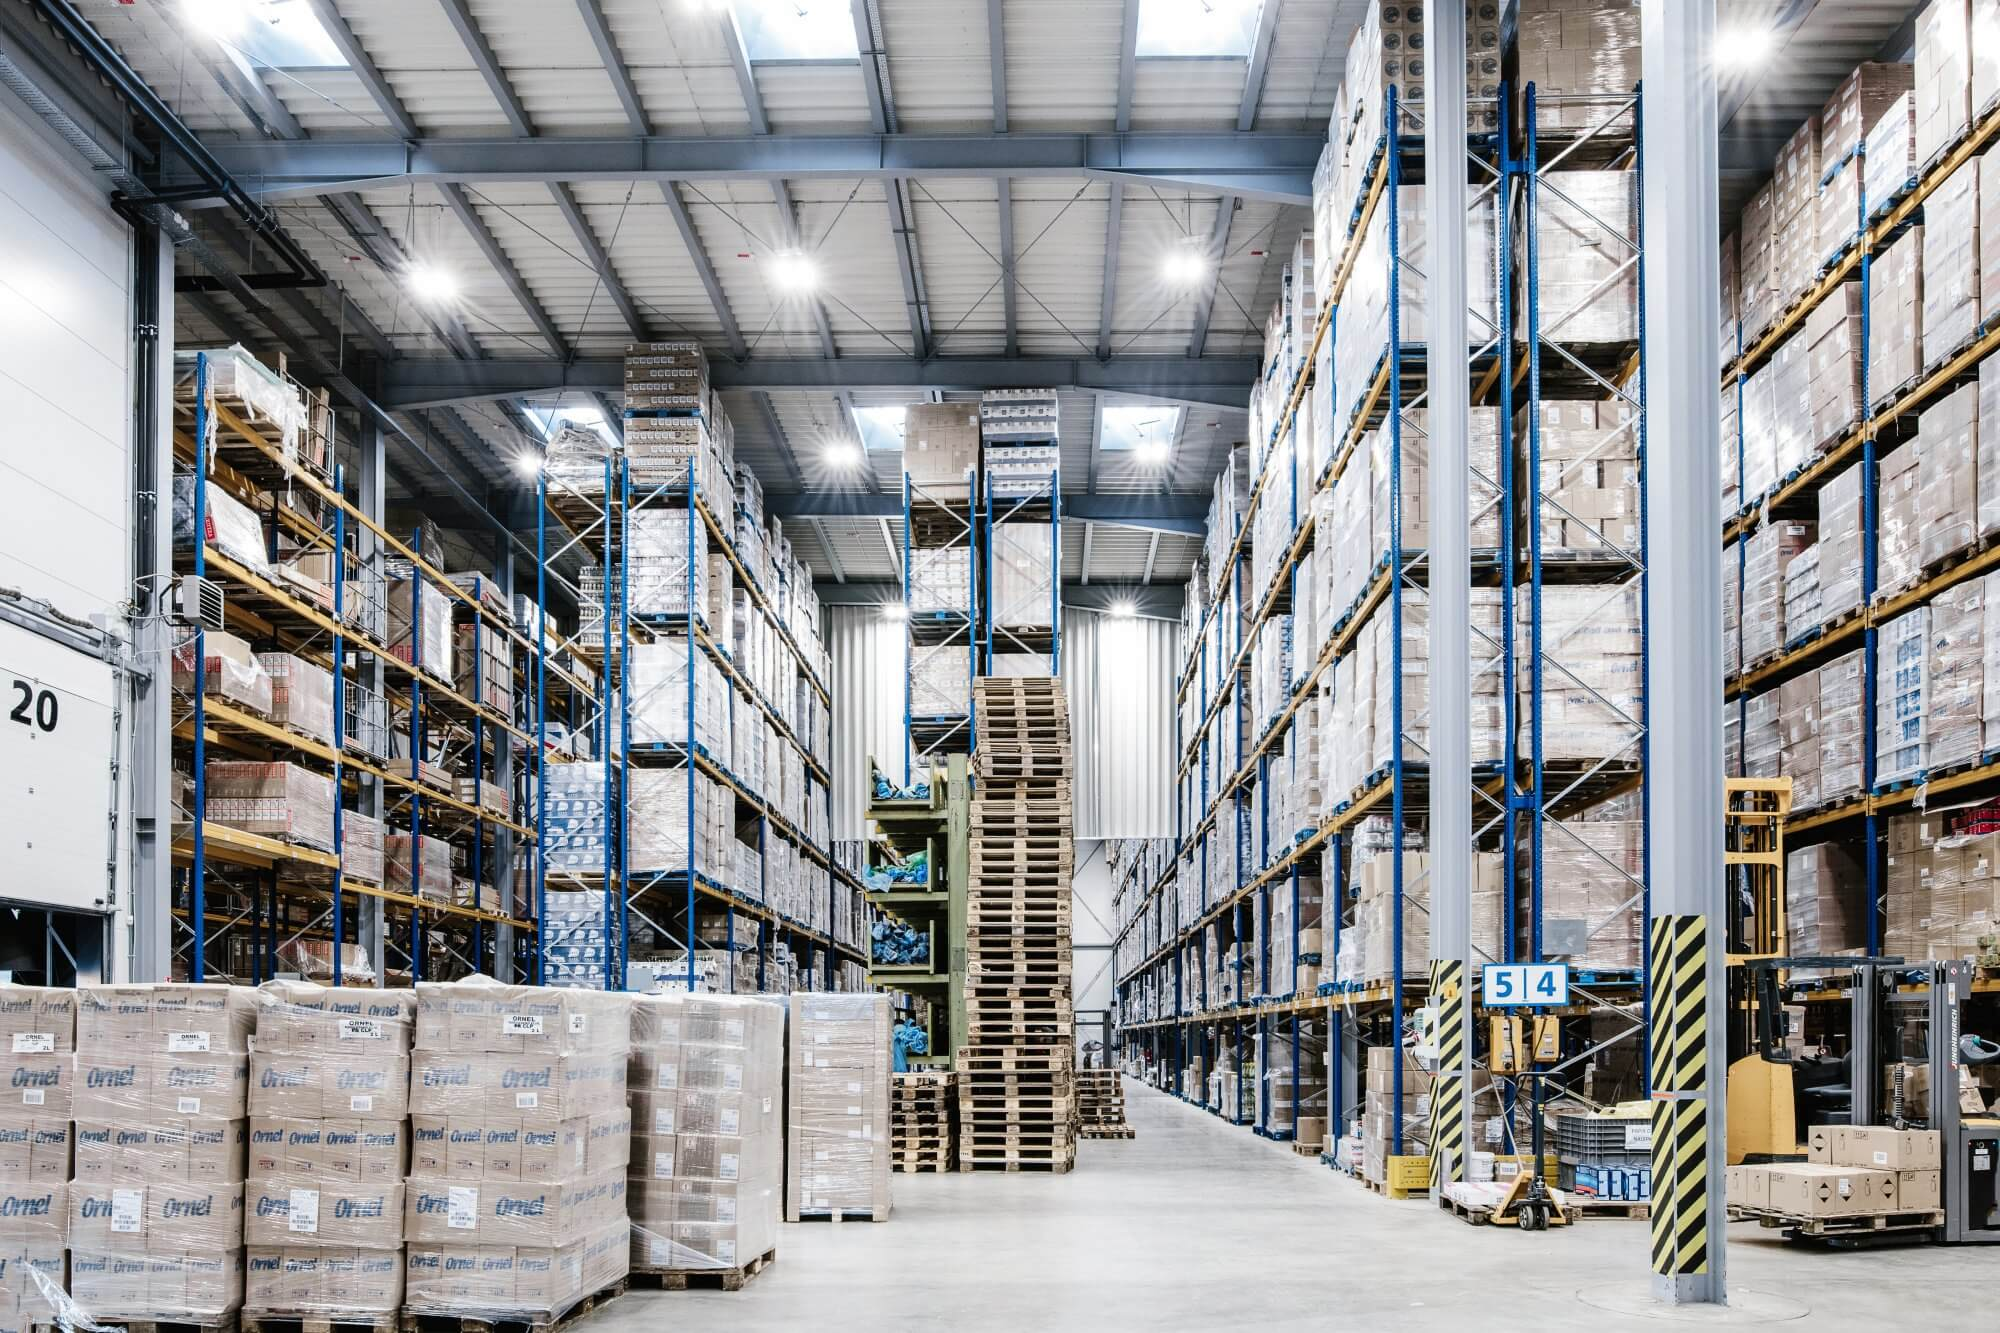
\includegraphics[width=10cm]{images/logisticki-centar.jpg}
    \caption{Logistički centar \citep{SmartSimply}.}
\end{figure}
\end{frame}

\begin{frame}
\frametitle{Uvod (2)}
\begin{figure}[htb]
    \centering
    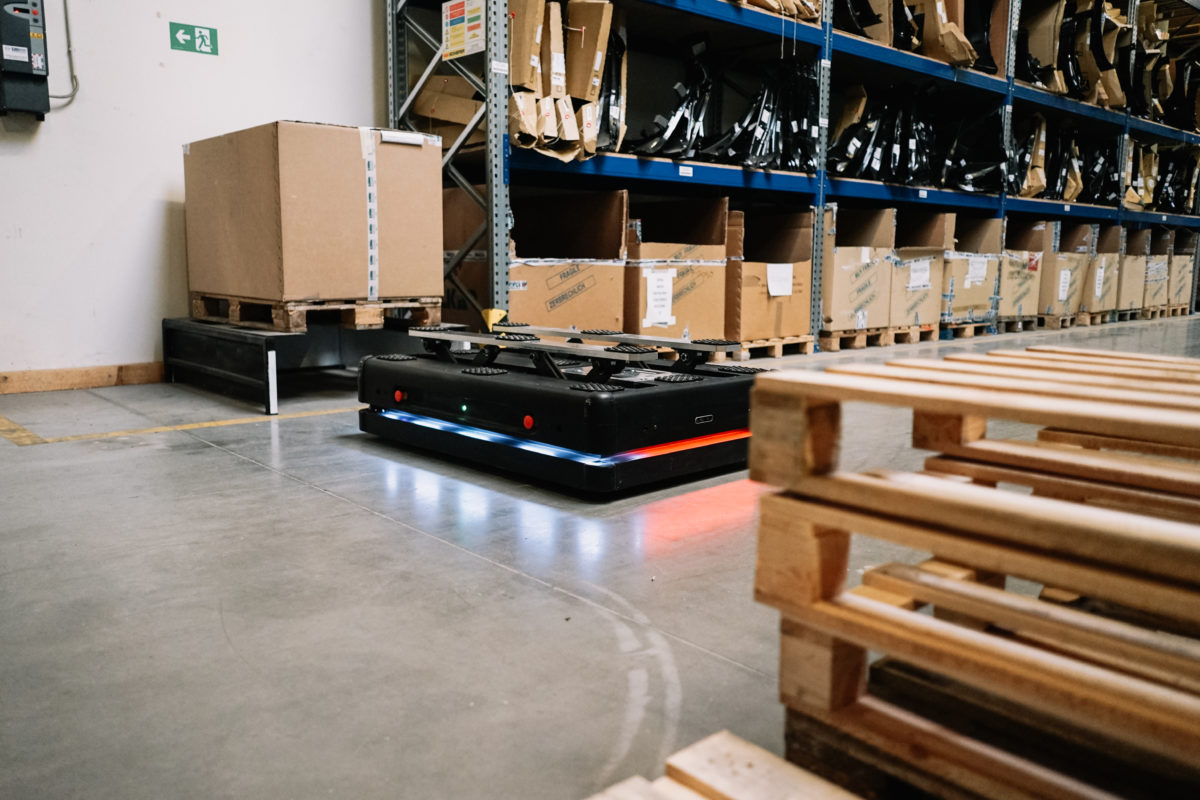
\includegraphics[width=10cm]{images/robot-01.jpg}
    \caption{Autonomni mobilni robot hrvatske tvrtke Gideon Brothers \citep{Gideon:Logisticsrobotlingo}.}
\end{figure}
\end{frame}

\section{Formalan opis problema raspoređivanja heterogene flote}
\begin{frame}
\frametitle{Formalan opis problema raspoređivanja heterogene flote}
\begin{figure}[htb]
    \centering
    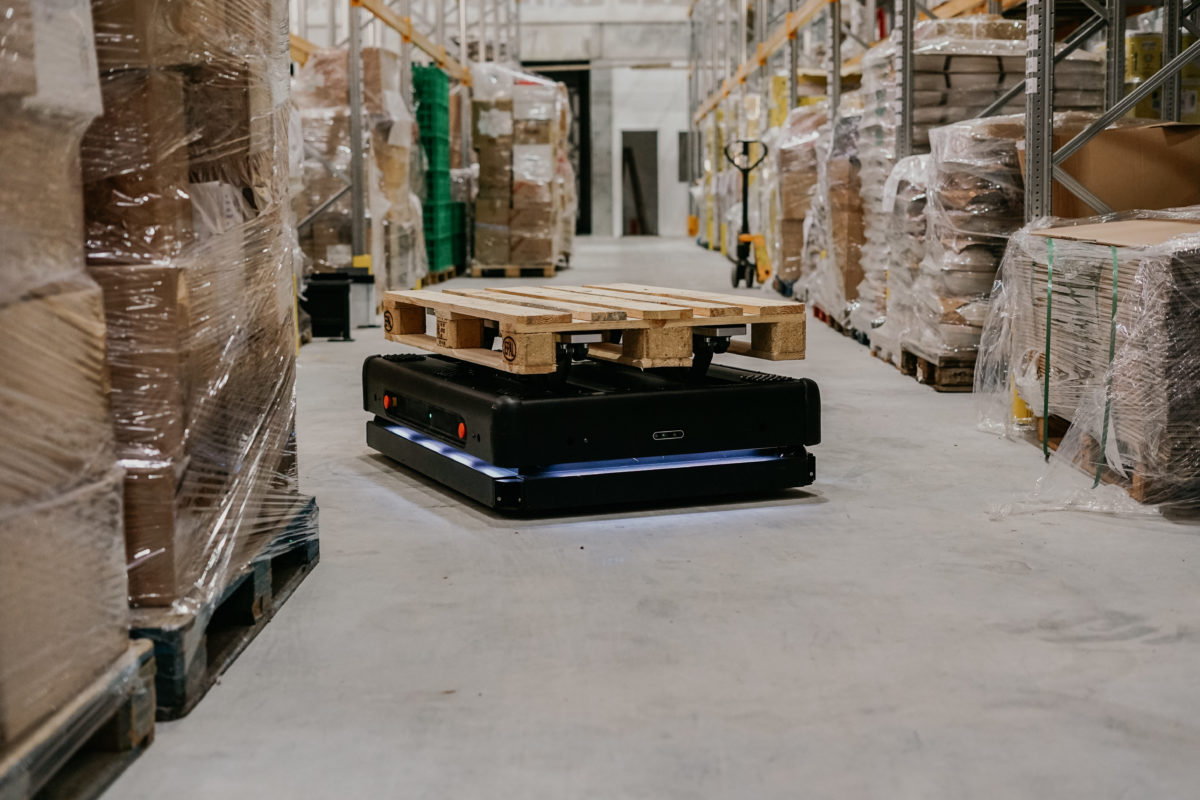
\includegraphics[width=10cm]{images/robot-02.jpg}
    \caption{Robot s praznom paletom, koji može započeti izvršavati narudžbu. \citep{Gideon:PollDebunks}.}
\end{figure}
\end{frame}

\subsection{Definicija heterogene flote}
\begin{frame}
\frametitle{Formalan opis problema raspoređivanja heterogene flote}
\framesubtitle{Definicija heterogene flote}
Heterogena flota sastoji se od $N_p$ ($1 \le N_p \le 25$) ljudi i
 $N_r$ ($1 \le N_r \le 50$) robota,
koji se mogu kretati u po skladištu širine $W$ ($W \in \mathbb{N},\ 1 \le W \le 4500$)
i  dužine $L$ ($L \in \mathbb{N},\ 1 \le L \le 4500$).
Skladište se može prikazati kao skup točaka:
\begin{equation}
S = \left\{(x, y)\ |\ x, y \in \mathbb{N}\ \land\ 1 \le x \le W\ \land\ 1 \le y \le L\right\},
\end{equation}
\begin{itemize}
    \item[$\bullet$] $M_i$ ($0 \le i < N_p$) - označava poziciju i-tog čovjeka,
    \item[$\bullet$] $R_i$ ($0 \le i < N_r$) - označava poziciju i-tog robota,
    \item[$\bullet$] $d_m(A, B)$ - označava vrijeme koje je potrebno čovjeku da od točke $A$ dođe do točke $B$ i obrnuto,
    \item[$\bullet$] $d_r(A, B)$ - označava vrijeme koje je potrebno robotu da od točke $A$ dođe do točke $B$ i obrnuto.
\end{itemize}
\end{frame}

\subsection{Definicija artikala i narudžbe}
\begin{frame}
\frametitle{Formalan opis problema raspoređivanja heterogene flote}
\framesubtitle{Definicija artikala i narudžbe}
Skup svih artikala $I$ zapravo je skup svih pozicija na kojima se artikli nalaze:
\begin{equation}
I = \left\{A, A \in S\right\}.
\end{equation}
$I_i$ ($0 \le i < |I|$) označava i-ti artikl u skupu $I$.

Narudžba $O_k$ definirana
je kao skup dvojki $(i, t_{i})$, gdje je $t_{i}$ vrijeme koje je potrebno
da čovjek stavi artikl $I_i$ na robota kada robot izvršava narudžbu $O_k$:
\begin{equation}
O_k = \left\{ (i, t_{i})\ |\ i \in 2^{\left\{0, 1, ..., |I|-1\right\}}\backslash\left\{\emptyset\right\},\ t_{i} \in \mathbb{R}_{\ge0}\right\}.
\end{equation}
\end{frame}

\subsection{Opis stanja skladišta}
\begin{frame}
\frametitle{Formalan opis problema raspoređivanja heterogene flote}
\framesubtitle{Opis stanja skladišta}
\end{frame}

\subsection{Ulazni podaci}
\begin{frame}
\frametitle{Formalan opis problema raspoređivanja heterogene flote}
\framesubtitle{Ulazni podaci}
\begin{itemize}
    \item Formatirano stanje skladišta.
    \item Sustav će na ulaz dobiti novo stanje skladišta nakon svake nove pristigle narudžbe.
    \item Budući da narudžbe pristižu stohastički onda se ne zna niti koliko često će sustav dobivati novo stanje skladišta na temelju kojega treba donesti nove odluke.
\end{itemize}
\end{frame}

\subsection{Očekivani izlazni podaci}
\begin{frame}
\frametitle{Formalan opis problema raspoređivanja heterogene flote}
\framesubtitle{Očekivani izlazni podaci}
\begin{itemize}
    \item Od sustava se očekuje da za svakog robota odredi narudžbe koje će izvršiti.
    \item Od sustava se očekuje da za svaki artikl odredi koji čovjek će ga staviti na pripadajućeg robota.
\end{itemize}
\end{frame}

\subsection{Ocjena kvalitete}
\begin{frame}
\frametitle{Formalan opis problema raspoređivanja heterogene flote}
\framesubtitle{Ocjena kvalitete}
Na temelju odluke sustava gradi se raspored čija kvaliteta \engl{fitness} je tim
veća što je prosječno vrijeme izvršavanje narudžbe manje. Ako s
$t_{s, i}$ označimo vrijeme početka izvršavanja narudžbe $i$, a s $t_{e, i}$
vrijeme završetka izvršavanja narudžbe $i$, onda je prosječno vrijeme izvršavanja
narudžbe jednako:
\begin{equation}
    \overline{T} = \sum_{i = 0}^{|O| - 1}{t_{e, i} - t_{s, i}},
\end{equation}
a kvaliteta rasporeda $f$ jednaka je $f = \overline{T}^{-1}$. Cilj je
pronaći takav raspored koji će minimizirati $\overline{T}$, odnosno
maksimizirati $f$.
\end{frame}

\section{Raspoređivanje}
\begin{frame}
\frametitle{Raspoređivanje (2)}
Raspoređivanje određuje raspodjelu resursa zadacima u zadanom vremenskom
intervalu s ciljem optimizacije jednog ili više kriterija \citep{michael2018scheduling}.
\vspace{0.5cm}

Resursi i zadaci su opisani različitim karakteristikama koje su bitne za raspoređivanje.
\vspace{0.5cm}
\begin{itemize}
    \item resursi, strojevi ili sredstva
    \item zadaci, poslovi ili aktivnosti
    \item \textit{online} i \textit{offline}
    \item statički (deterministički) i dinamički (stohastički)
\end{itemize}
\end{frame}

\begin{frame}
\frametitle{Raspoređivanje (2)}
U svim problemima raspoređivanja pretpostavlja se da je
broj poslova $n$ i broj strojeva $m$ konačan. Oznakom $j$ najčešće se
označava posao, a s $i$ stroj. Poslovi su najčešće opisani sljedećim
informacijama:
\begin{itemize}
    \item[$\bullet$] $p_{ij}$ - vrijeme izvršavanja posla $j$ na stroju $i$,
    \item[$\bullet$] $r_{j}$ - vrijeme u kojem posao $j$ postane raspoloživ za raspoređivanje,
    \item[$\bullet$] $d_j$ - vrijeme željenog završetka i
    \item[$\bullet$] $w_j$ - prioritet posla.
\end{itemize}
\end{frame}

\subsection{Metode rješavanje problema raspoređivanja}
\begin{frame}
\frametitle{Raspoređivanje}
\framesubtitle{Metode rješavanja problema raspoređivanja}
\begin{itemize}
    \item NP-teški problemi.
    \item Heurističke metode koje ne pronalaze nužno optimalno rješenje.
    \item Algoritmi koji pretražuju prostor stanja (statička \textit{offline} okruženja)
    \begin{itemize}
        \item genetski algoritmi, simulirano kaljenje, optimizacija rojem čestica, mravlja algoritam, itd.
    \end{itemize}
    \item Algoritmi koji grade rješenje izravno (dinamička \textit{online} okruženja)
    \begin{itemize}
        \item Na temelju stanja sustava određuju kako raspodijeliti pojedini posao.
    \end{itemize}
\end{itemize}
\end{frame}

\section{Raspoređivanje heterogene flote}
\begin{frame}
\frametitle{Raspoređivanje heterogene flote}
U DRCFJSP problemu na raspolaganju je skup od $n$ nezavisnih poslova $J = \left\{J_1, J_2, ..., J_n\right\}$,
zatim skup od $m$ strojeva $M = \left\{M_1, M_2, ..., M_m\right\}$, i skup od $l$ radnika $W = \left\{W_1, W_2, ..., W_l\right\}$.
Svaki posao ima $r$ operacija $\left\{O_{i,1}, O_{i,2}, ..., O_{i,r}\right\}$ Svakim strojem $M_i$
mora upravljati neki radnik iz skupa $W$
\end{frame}

\section{Zaključak}
\begin{frame}
\frametitle{Zaključak}
\end{frame}

\begin{frame}
\frametitle{Literatura}
\bibliography{literatura}
\bibliographystyle{fer}
\end{frame}

\end{document}
